  
\documentclass[titlepage,a4paper]{article}

\usepackage{a4wide}
\usepackage[colorlinks=true,linkcolor=black,urlcolor=blue,bookmarksopen=true]{hyperref}
\usepackage{bookmark}
\usepackage{fancyhdr}
\usepackage[spanish]{babel}
\usepackage[utf8]{inputenc}
\usepackage[T1]{fontenc}
\usepackage{graphicx}
\usepackage{float}

\pagestyle{fancy} % Encabezado y pie de página
\fancyhf{}
\fancyhead[L]{TP1S - Max Mustermann}
\fancyhead[R]{Algoritmos y Programación III - FIUBA}
\renewcommand{\headrulewidth}{0.4pt}
\fancyfoot[C]{\thepage}
\renewcommand{\footrulewidth}{0.4pt}

\begin{document}
\begin{titlepage} % Carátula
	\hfill
\includegraphics[width=6cm]{logofiuba.jpg}
    \centering
    \vfill
    \Huge \textbf{Trabajo Práctico 2 — Kahoot}
    \vskip2cm
    \Large [7507/9502] Algoritmos y Programación III\\
    Curso 1 \\ % Curso 1 para el de la tarde y 2 para el de la noche
    Primer cuatrimestre de 2020
    \vfill
    \begin{tabular}{ | l | l | l |} % Datos del alumno
      \hline
      Alumno & Padron & Mail \\ [0.5ex] 
      \hline\hline
     Agustin Brasburg & 104733 & abrasburg@fi.uba.ar\\ 
     \hline
     Damian Ganopolsky & 101168 & dganopolsky@fi.uba.ar\\
     \hline
     Andres Jalife & 104342 & ajalife@fi.uba.ar \\
     \hline
    Maximiliano Levi & 104288 & mlevif@fi.uba.ar \\
     \hline
     Mathias Welz & 101552 & mwelz@fi.uba.ar \\ [1ex] 
     \hline
  	\end{tabular}
    \vfill
    \vfill
\end{titlepage}

\tableofcontents % Índice general
\newpage

\section{Introducción}\label{sec:intro}
El presente informe reune la documentación de la solución del segundo trabajo práctico de la materia Algoritmos y Programación III que consiste desarollar un juego de quiz que se asimila al Kahoot utilizando las tecnicas de Java, TDD y Git para lograr un trabajo grupal.

\section{Supuestos}\label{sec:supuestos}
% Deberá contener explicaciones de cada uno de los supuestos que el alumno haya tenido que adoptar a partir de situaciones que no estén contempladas en la especificación.
\item[ExtensionInvalidaExcepcion]

\section{Modelo de dominio}\label{sec:modelo}
% Explicación concisa del diseño general del trabajo.

\section{Diagramas de clase}\label{sec:diagramasdeclase}
% Uno o varios diagramas de clases mostrando las relaciones estáticas entre las clases.  Puede agregarse todo el texto necesario para aclarar y explicar su diseño. Recuerden que la idea de todo el documento es que quede documentado y entendible cómo está implementada la solución.

Kahoot es la clase encargada de empezar el juego y guardar el panel que muestra el juego, las preguntas que se mostraran con sus respectivas respuestas y puntos por responder bien, y sus jugadores con sus respectivos nombres, puntaje y modificadores de puntajes.

\begin{figure}[H]
\centering
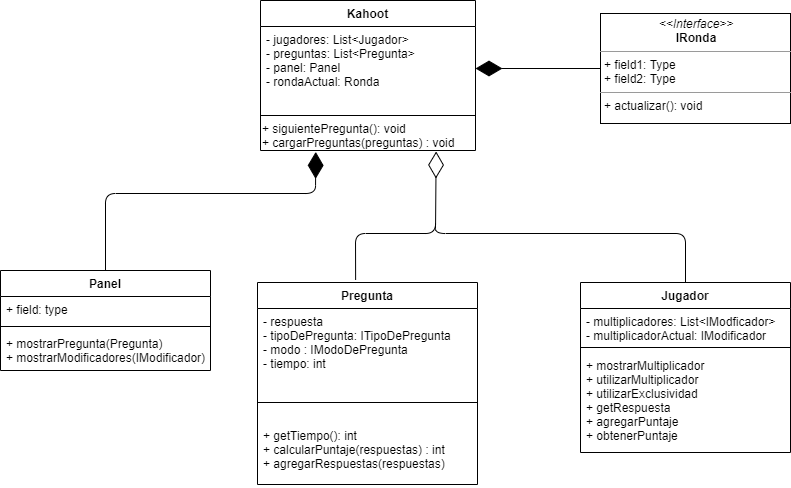
\includegraphics[width=0.8\textwidth]{diagramaGeneral.png}
\caption{\label{fig:class01}Diagrama del Kahoot.}
\end{figure}

\begin{figure}[H]
    \centering
    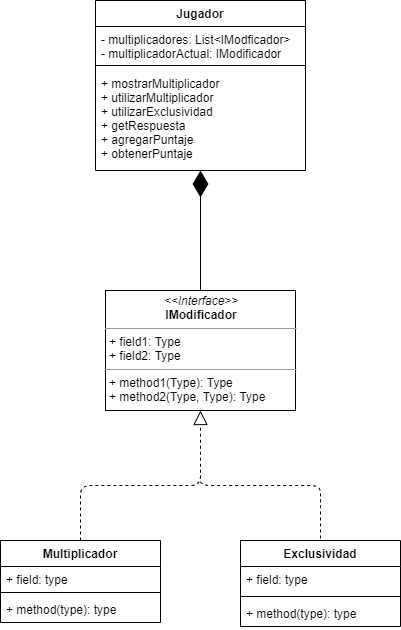
\includegraphics[width=0.8\textwidth]{diagramaJugador.png}
    \caption{\label{fig:class02}Diagrama del Jugador.}
\end{figure}

\begin{figure}[H]
    \centering
    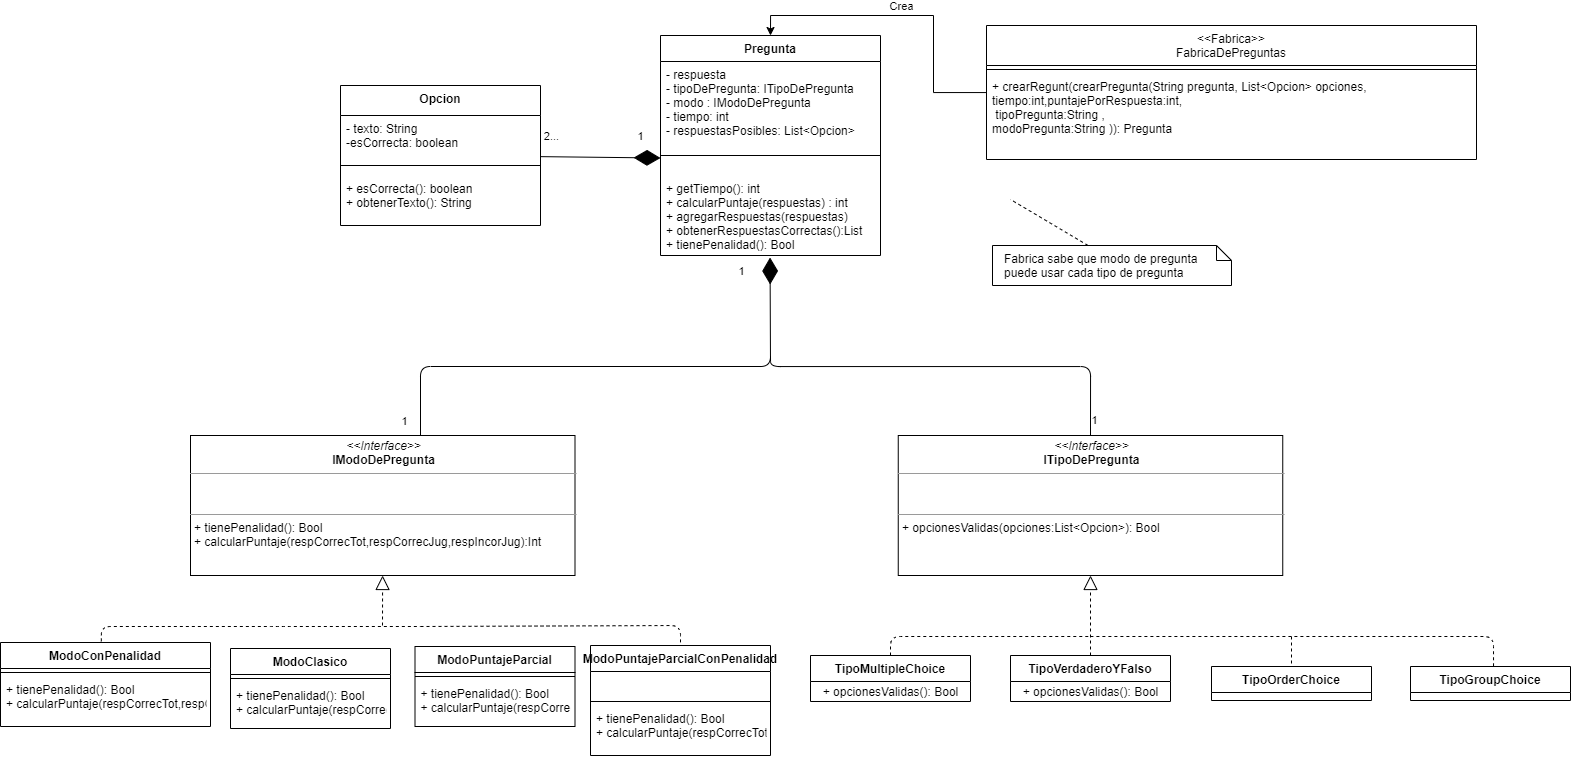
\includegraphics[width=0.8\textwidth]{diagramaPregunta.png}
    \caption{\label{fig:class03}Diagrama de Pregunta.}
\end{figure}

\begin{figure}[H]
    \centering
    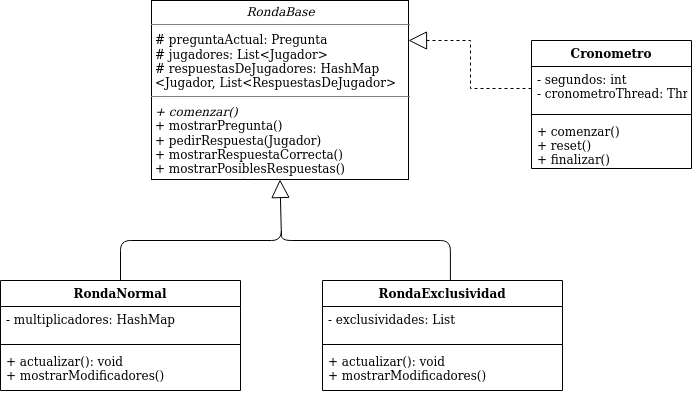
\includegraphics[width=0.8\textwidth]{diagramaRonda.png}
    \caption{\label{fig:class04}Diagrama de Ronda.}
\end{figure}


\section{Detalles de implementación}\label{sec:implementacion}
% Explicaciones sobre la implementación interna de algunas clases que consideren que puedan llegar a resultar interesantes.

\subsection{Inicializacion de preguntas}
Actualmente le proveemos dos formas distintas de cargar las preguntas al programa.

\begin{description}
{\bf Formato Propio}\newline
El archivo con el que inicializamos las preguntas contenia las lineas con el siguiente formato Modo/Tipo/Pregunta/Opciones/OpcionCorrecta .\newline
\newline

Siendo el contenido de cada campo el siguiente:\newline
\newline

Modo: String\newline
\indent- ConPuntajePenalidad\newline
\indent- Clasico\newline
\indent- Parcial\newline
\newline

Tipo: String\newline
\indent- MultipleChoice\newline
\indent- VerdaderoFalso\newline
\indent- OrderedChoice\newline
\indent- GroupChoice\newline
\newline

Pregunta: String\newline
\newline
Opciones: String,String,String\newline
\newline
OpcionCorrecta: String\newline
\newline

Ejemplo:\newline
\begin{verbatim}
Clasico/MultipleChoice/¿Como se llama tu mascota?/Nestor,Chewbacca,Godzilla/Godzilla
\end{verbatim}
\newline

\end{description}

\begin{description}
{\bf Formato JSON}

\newline
\newline
El formato JSON mantiene la misma idea de formato propio, representando a los modos, las opciones y las preguntas como strings pero la diferencia principal es que estan separadas por categorias y que se utilizan los arrays que provee el formato JSON

\newline
\newline
Ejemplo
\begin{verbatim}
{
  "MultipleChoice" :
      [{
        "modo": "ConPuntajeParcial",
        "texto" : "¿Quién gano gran hermano 2015?",
        "opciones" : ["Matías Schrank", "Francisco Delgado", "Vos"],
        "opcionesCorrectas": ["Francisco Delgado"],
      }]
}
\end{verbatim}
\end{description}

\subsection{Proin sodales leo dapibus sapien fermentum}
Quisque tempus, tortor et convallis interdum, ipsum leo tempus ipsum, in molestie tortor arcu sit amet tellus. Praesent fermentum hendrerit nulla. In maximus ornare maximus. Nullam consectetur placerat enim sit amet lacinia. Etiam pellentesque tellus consectetur hendrerit iaculis. Sed non laoreet felis.

\section{Excepciones}\label{sec:excepciones}
% Explicación de cada una de las excepciones creadas y con qué fin fueron creadas.

\begin{description}
\item[ExtensionInvalidaExcepcion] Esta excepcion fue creada con el fin de notificar al usuario que el archivo de preguntas que se dio tiene una extension erronea.
\item[NoQuedanUsosExcepcion] Esta excepcion fue creada con el fin de notificar al usuario que el Multiplicador que se utilizo no tenia usos disponibles y por ende la ejecucion no puede continuar.
\end{description}

\section{Diagramas de secuencia}\label{sec:diagramasdesecuencia}
% Mostrar las secuencias interesantes que hayan implementado. Pueden agregar texto para explicar si algo no queda claro.

\begin{figure}[H]
\centering
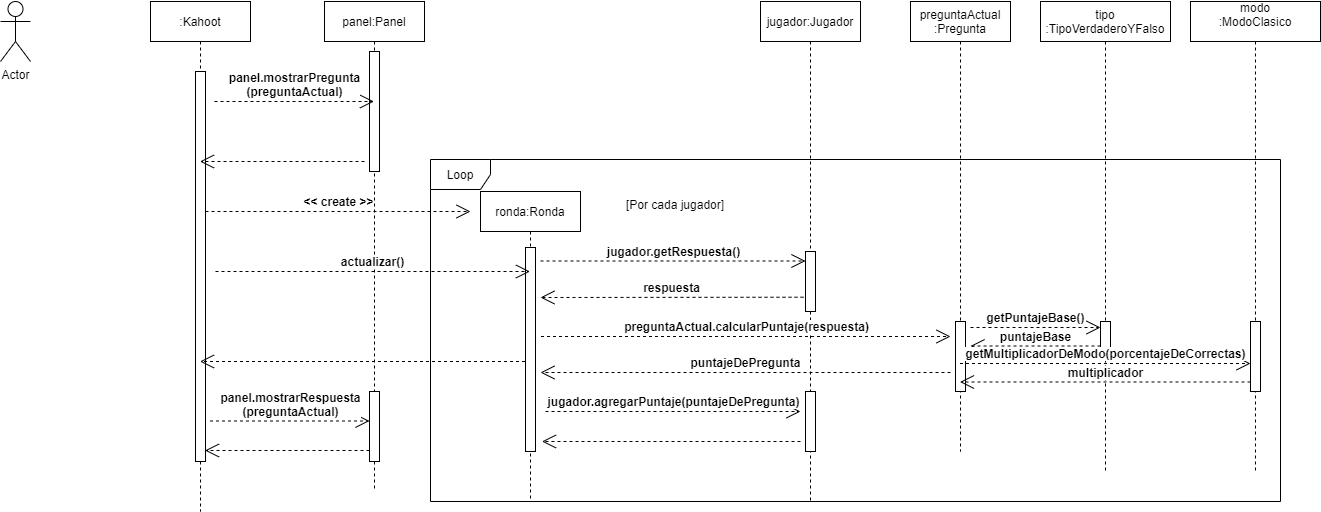
\includegraphics[width=0.8\textwidth]{diagramaDeSecuencia.png}
\caption{\label{fig:seq01}Se muestra el proceso de una ronda en el que un jugador responde una pregunta, se calcula el puntaje y se le agregan los puntos obtenidos.}
\end{figure}

\section{Diagrama de paquetes}\label{sec:diagramasdepaquetes}

Incluir un diagrama de paquetes UML para mostrar el acoplamiento de su trabajo.

\section{Diagramas de estado}\label{sec:diagramasdeestados}

Incluir diagramas de estados, mostrando tanto los estados como las distintas transiciones para
varias entidades del modelo.

\end{document}
